\documentclass[12pt]{article}

\usepackage[utf8]{inputenc}
\usepackage{color}
\usepackage{graphicx}

\title{Manual Básico de LaTeX}
\author{
	Elyas Correa Nogueira\\
	\and
	Fabiana Silva Finoti\\
	\and
	Isabela Daiana Pereira\\
	\and
	Israel Mateus Melo Oliveira\\	
}
\date{6 de Maio de 2019}

\begin{document}
	
	\maketitle
	
	\newpage
	
	\section{Introdução}
	O Latex (estilizado como \LaTeX) é um sistema de preparação de documentos desenvolvido nos anos 80 pelo americano Leslie Lamport. Amplamente empregado na fabricação de documentos, o LaTeX utiliza texto simples para a confecção dos arquivos, fazendo a formatação do texto (\textit{itálico}, \textbf{negrito} {\color{red} cores}) por meio de marcadores, de maneira que o escritor foque no conteúdo ao invés da estilização.
	
	A padronização dos documentos oferecidos pelo LaTeX faz com que ele seja preferencial na fabricação de vários documentos acadêmicos, eliminando assim erros na formatação de tais documentos. Neste manual, será abordada a estrutura básica de um documento TeX e vários pacotes que oferecem funcionalidades importantes para quem está escrevendo o documento.
	
	\section{Como utilizar o LaTeX?}
	
		\subsection{Instalação em Linux e Windows}
		
			\subsubsection{Instalação em Ubuntu}
			Para facilitar o processo, será explicado como instalar o LaTeX em um sistema Ubuntu. Abra o terminal e digite a seguinte linha:\\\\
			\texttt{sudo apt-get install texlive texlive-latex-extra texlive-lang-portuguese}\\
			
			Assim, será instalado em seu computador os pacotes necessários para compilar arquivos básicos .tex. Para o uso de ferramentas mais complexas, pode ser necessária a instalação de outros pacotes -- como o \texttt{texlive-math-extra}, usado para matemática complexa. 
			
			Uma vez que os pacotes de compilação foram instalados, você precisará de um editor para começar a sua aventura LaTeX. Para respeitar o que foi utilizado em aula, é recomendado que você use o TeXstudio. Para instalá-lo, abra o terminal e digite:\\\\
			\texttt{sudo apt-get install texstudio}
			
			\subsubsection{Instalação em Windows}
			No Windows, a instalação dos compiladores e do editor podem ser feitas por meio do browser. Entre no link \texttt{https://miktex.org/download}, tenha certeza que você está na aba do Windows e clique no botão de Download (o site oferece um tutorial passo-a-passo em caso de dúvidas). Quando o arquivo for baixado, abra o instalador, faça bom uso do 'Avançar' e espere o fim do processo.
			
			Agora que os compiladores estão instalados, chegou a hora do editor. Entre no link \texttt{http://texstudio.sourceforge.net/}, clique na aba de Downloads, ache a versão correspondente ao seu Windows e espere o fim do download. Abra o instalador e vá clicando em 'Avançar' até que o TeXstudio esteja instalado em seu computador.
			
		\subsection{Criação de Documento Básico}
		
			Nessa subseção, você será apresentado a um código básico de LaTeX e as linhas serão explicadas posteriormente.
			
			\begin{figure}[h]
				\begin{center}
					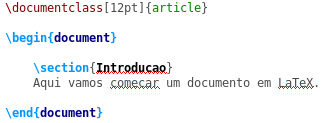
\includegraphics{codigo1.png}
				\end{center}
			\end{figure}
		
		    Na primeira linha, o escritor declara que o documento digitado será do tipo \textit{article}, ou seja, seguirá os padrões de formatação de um artigo acadêmico.
			
			
			
		
	
\end{document}